
\chapter{Error messages and problem resolutions}
\label{chap:error_messages}

\section{Error message 1}

\subsection{Problem identification}
When I try to log in through the iCrash admin system, it doesn't accept that
which is written in the readme file.

\subsection{Corrective actions}
1. The simplest way to know if all the VM are up and running is looking at the
messages that appear after you type vagrant up \\
2. Other thing you could try is to type in your console: vagrant box list .It
shows the different vagrant boxes already downloaded in your machine.\\
3. Also in case of using Vagrant project you need to check if all virtual
machines were started correctly. In particular you should login into the server VM and see if the server has been started: you can do it by typing:  ps -ax | grep java which displays all Java processes running on the machine.



\section{Error message 2}

\subsection{Problem identification}
I made iCrash project changes in order to implement the variants. Before
changing I could start the project but after modifications, an error is
displayed. I think maybe this is an error in the server.\\

\begin{figure}
\begin{center}
\includegraphics[width=0.5\textwidth]{./images/er1.eps}
\end{center}
\caption{Error message - problems with log-in}
\end{figure}

\subsection{Probable cause}
This problem may happen because you made a copy of the iCrash project into the
same workspace (let's say you decided to called iCrash2), but you did not change
the Web Project settings configuration\\

\subsection{Corrective actions}
Right-click on the project->properties, then select Web Project Settings. You
need to change the context root to a name other than iCrash (maybe iCrash2).\\
In case you still have problems to run the web application, have a look into the file server.xml, placed inside the Servers project, into the folder Tomcat v8.0 Server. Search for the entries "Context" and ensure that the property path points to the right context for each entry appearing into the file.
 

\section{Error message 3}

\subsection{Problem identification}
I would like to modify a class in iCrash H5, whose GUI was created with Vaadin
Designer, but it looks broken and is unmodifiable. What could I do?\\

\begin{figure}
\begin{center}
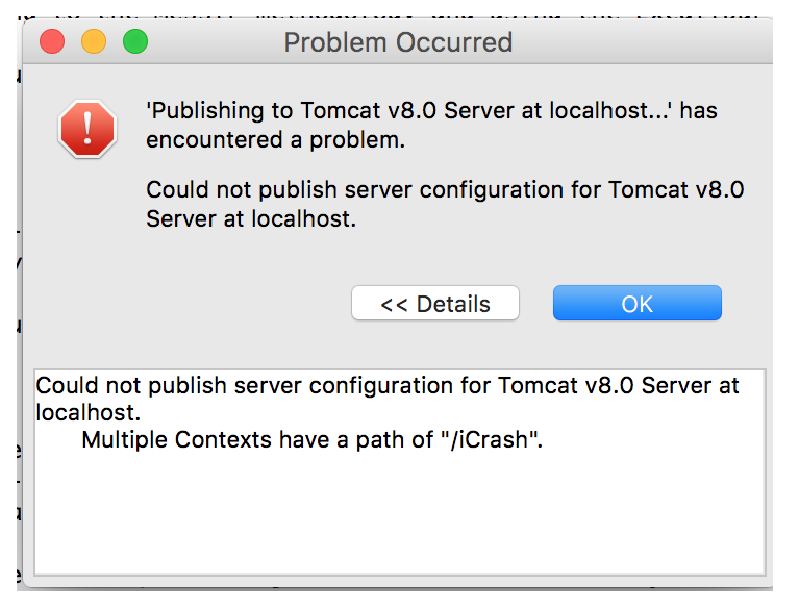
\includegraphics[width=0.5\textwidth]{./images/er2.eps}
\end{center}
\caption{Error message - problems with GUI}
\end{figure}

\subsection{Probable cause}
GUI might not be supported by your drivers.
 
\subsection{Corrective actions}
Method 1: 
You need to change ComCompanyDesign's theme from icrash to valo.
It then solves the problem:

\begin{figure}
\begin{center}
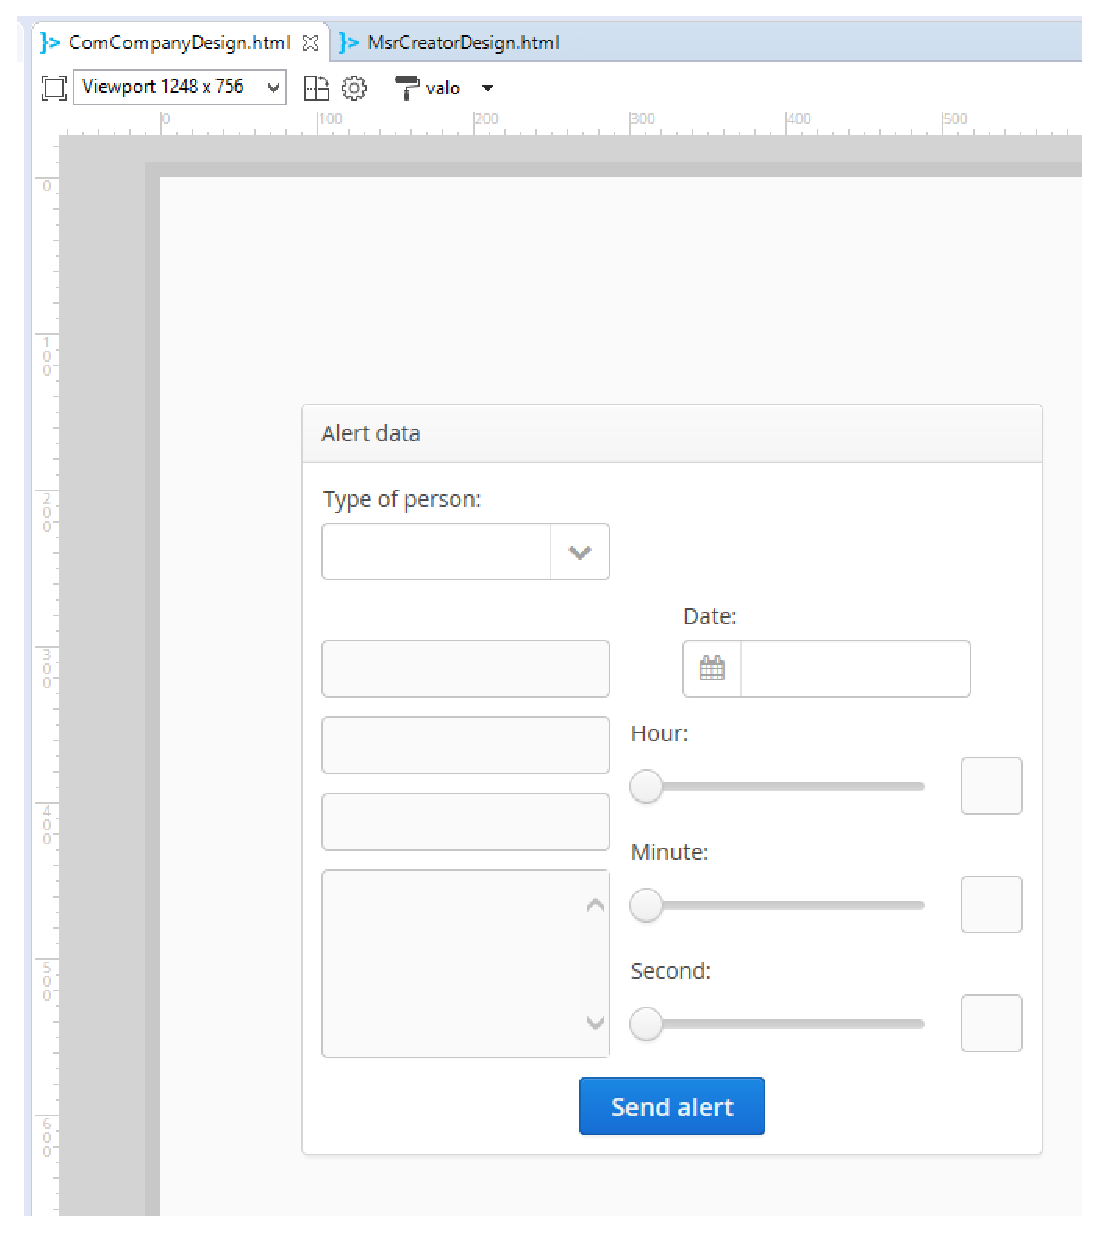
\includegraphics[width=0.5\textwidth]{./images/er3.eps}
\end{center}
\caption{Error message - solution to GUI}
\end{figure}

Method 2:\\
Unzip 1.zip to project's WebContent VAADIN-themes-icrash\\
Clean the project (build automatically should be on) and reopen ComCompanyDesign.
You will then get the same result with icrash theme - the design will become editable.


\section{Error message 4}

\subsection{Problem identification}
When compiling a message indicates that there is a file missing.

\subsection{Probable cause}
Issues with correct PATH.

\subsection{Corrective actions}
You need to ensure that:\\
1) you are using Excalibur v1.5.1\\
2) you have the latest version of the Excalibur Standard Libraries setup in your
environment, If not sure, then remove the projects from the workspace, and then
add them again.\\ 3) you have the latest released iCrash Specification in your
workspace. If not sure, then remove the project from the workspace and add it
again. \\
Once you have ensured the previous steps, check if the problem remains.


\section{Error message 5}

\subsection{Problem identification}
Is it normal that all the views (even the ones that come with the icrash
specification project) and their documentation are missing? Is there a way to recover the views that come with the project and their captions?

\subsection{Probable cause}
Problems with displaying data.

\subsection{Corrective actions}
No it is normal that all the original views of the icrash specification project
are missing and their documentation are missing.\\
1. Close Eclipse\\
2. You can copy/paste the following files from the original icrash project to
your icrash variant project.\\
2.a the representation.aird file\\
2.b all msrd files in the folder lu.uni.lassy.excalibur.examples.icrash/views"\\
3 Launch Eclipse\\

